\newgeometry{top=3cm, bottom=2cm}
\chapter{Results}
\label{chapter:results}

This chapter covers the results and analysis of the case study. First the results of interview for demographic purposes are
presented. Second, survey and interview results regarding JUnit compared to Spock and Spectrum are analyzed.  Third, the test
code analysis is presented and finally
with all the above mentioned results, Spock and Spectrum are compared against each other.


%-Define the population to which inferential statistics and predictive models apply.\newline
%-RQ1 and RQ2 answered by comparing initial and post surveys\newline
%-Comparing Spock and Spectrum vs each other\newline
%-RQ3 answered by comparing observed actual test implementation changes\newline

\section{First interview: Demographics and projects}
\label{section:demographics}
    First interview was conducted to study about the demographics of participants and projects under research.
    The demographics of participants are displayed in table \ref{tab:demographics}. To summarize the
    participants, all can be categorized as senior software developers with many years of working with \textit{xUnit testing family} frameworks.
    Only participant C has a fair amount of prior experience working with BDD testing frameworks.
    \begin{table}[H]
        \resizebox{\textwidth}{!}{%
            \begin{tabular}{p{8.0cm}*{3}{p{3.5cm}}}
            \headcol & & &  \\
            \headcol {\large\textbf{Participant attribute}} & {\large\textbf{Participant A}} & {\large\textbf{Participant B}} & {\large\textbf{Participant C}} \\
            \hline
            \rowcol & & & \\
            \rowcol \textbf{Project} & Project A & Project A & Project B \\ \hline
            & & & \\
            \textbf{Software development experience} & 17 years & 15 years & 8 years \\ \hline
            \rowcol & & &  \\
            \rowcol \textbf{Java development experience} & 14 years & 1 year & 5-6 years  \\ \hline
            & & &  \\
            \textbf{Spring Framework experience} & 7 years & 1 year & 5-6 years \\ \hline
            \rowcol & & &  \\
            \rowcol \textbf{Automated unit testing experience} & 14 years; & 10 years; & 3-4 years; \\
            \rowcol \multicolumn{1}{r}{\textit{with frameworks}\textcolor{white}{-------------}} & \textit{JUnit} & \textit{CPPUnit, JUnit} & \textit{JUnit, TestNG} \\ \hline
            & & &  \\
            \textbf{Automated integration testing \newline experience} & 14 years; & Hardly at all; & 5-6 years; \\
            \multicolumn{1}{r}{\textit{with frameworks}\textcolor{white}{------------}} & \textit{JUnit, Some Robot Framework with Selenium} & \textit{JUnit} & \textit{JUnit, TestNG} \\ \hline
            \rowcol & & &  \\
            \rowcol \textbf{BDD testing framework experience} & \textless \textit{ } 1 year; & - & 2-3 years; \\
            \rowcol \multicolumn{1}{r}{\textit{with frameworks}\textcolor{white}{------------}} & \textit{Jasmine, Mocha} & & \textit{JBehave} \\
            \rowcol & & &  \\ \bottomlinec
            \end{tabular}}
            \caption {Participant demographics} \label{tab:demographics}
    \end{table}
\restoregeometry

The projects under study can both be categorized as web application projects with Java \textit{Spring Framework} backend technology.
They both have an agile development process. \textbf{Project A} is a customer project in public administration context.
\textbf{Project B} is an in-house project. They are both on the medium scale in code size, but financially project A can be
categorized as medium to large category.

Project A has two developers, \textbf{participants} A and \textbf{B}, working with Spring Framework backend,
where there is automated low-level testing in place with \textit{JUnit}.
Project B has only one backend developer, \textbf{participant C}, working with Spring Framework. As Project B
was developed in larger scale from 2012 to 2013 and published originally in 2013, it has some of the automated
low-level testing with JUnit done by others than participant C. Still most of this kind of test work is done by participant C.
Table \ref{tab:projects} displays the details of projects A and B.
    \begin{table}[H]
        \resizebox{\textwidth}{!}{%
            \begin{tabular}{p{7.5cm}*{2}{p{6cm}}}
            \headcol & & \\
            \headcol {\large\textbf{Project attribute}} & {\large\textbf{Project A}} & {\large\textbf{Project B}} \\ \hline
            \rowcol & &  \\
            \rowcol \textbf{Description} & Web application for area management, replacing existing system & Wep application for working hours tracking \& reporting \\ \hline
            & &   \\
            \textbf{Context} & Public administration, development for customer & In-house develoment \\ \hline
            \rowcol & & \\
            \rowcol \textbf{Development process} & Agile development with customized \textit{Scrum} & Agile with loosely defined process \\ \hline
            & &  \\
            \textbf{Size \& development team} & Medium - large project; \newline 3 developers for approximately 1,5 years & Small - medium project; \newline Published 2013, now 2 developers maintaining \& further development \\ \hline
            \rowcol & & \\
            \rowcol \textbf{Architecture} & Client rendered single-page \newline application & Server MVC with some client rendered views \\ \hline
            & & \\
            \textbf{Technologies} & \textit{Java Spring Boot \& Angular 2} & \textit{Java Spring Framework \& JSP, Backbone.js} \\ \hline
            \rowcol & & \\
            \rowcol \textbf{Quality assurance process} & Automated unit \& integration testing, code reviews, continuous integration, no dedicated tester & Automated unit, integration \& acceptance testing, code reviews, continuous integration, no dedicated tester \\ \hline
            & & \\
            \textbf{Used unit testing framework} & \textit{JUnit} & \textit{JUnit} \\ \hline
            \rowcol & &  \\
            \rowcol \textbf{Used integration testing framework} & \textit{JUnit} extended for \textit{Spring Framework} & \textit{JUnit} extended for \textit{Spring Framework} \\
            \rowcol & &  \\ \bottomlinec
            \end{tabular}}
            \caption {Project details} \label{tab:projects}
    \end{table}

\newgeometry{left=2cm, right=2cm}
\section{Surveys and BDD framework feedback interview analyzed}

\subsection{Automated low-level testing developer practices}

    \begin{table}[H]
        \resizebox{\textwidth}{!}{%
            \begin{tabular}{p{13.0cm}*{7}{p{2cm}}}
            \topline
            \textbf{Question} & \textbf{Answer options} &  &  &  &   &  & \\ \hline
            \textbf{Q1: How do you spend your software development time (in percentages)} & Participant {\colorbox{lightgray}A} & Participant {\colorbox{lime}B} & Participant {\colorbox{orange}C} & Average & & \\
            & & & & & & & \\
            1. Writing new code & 20\% & 40\% & 15\% & 25\%  \\
            2. Writing new tests & 20\% & 25\% & 20\% & 21.67\% \\
            3. Debugging/fixing & 30\% & 25\% & 25\% & 26.67\% \\
            4. Refactoring & 20\%  & 10\% & 30\% & 23.33\% \\
            5. Other & 10\% & 0\% & 10\% & 6.67\% \\
            & \\ \hline
            \textbf{Q1': Compared to JUnit, How do you spend your software development time?} & A lot less time & Less time & Slightly less time & The Same amount of time & Slightly more time & More time & A lot more time \\
            & \\
            1. Writing new code & 0 & 0 & 0 & {\colorbox{lightgray}A} & 0 & 0 & 0 \\
            2. Writing new tests & 0 & 0 & 0 & {\colorbox{lightgray}A} & 0 & 0 & 0 \\
            3. Debugging/fixing & 0 & 0 & 0 & {\colorbox{lightgray}A} & 0 & 0 & 0 \\
            4. Refactoring & 0 & 0 & 0 & {\colorbox{lightgray}A} & 0 & 0 & 0 \\
            5. Other & 0 & 0 & 0 & {\colorbox{lightgray}A} & 0 & 0 & 0 \\
            & \\ \hline

            \textbf{Q2: How do you spend your low-level automated testing time} & Participant {\colorbox{lightgray}A} & Participant {\colorbox{lime}B} & Participant {\colorbox{orange}C} & Average & & \
            & & & & & & & \\
            1. How much approximately you use time per test case (minutes)? & 30 min & 30 min & 30 min & 30 min \\
            2. How much of your initial effort goes to thinking about test case content without implementation (percentage)? & 50\% & 20\% & 15\% & 28.33\% \\
            3. How much of your initial effort goes to initial test case structuring and implementation (percentage)? & 50\% & 80\% & 85\% & 71.67\% \\
            4. How much of your overall testing effort goes to refactoring test code (percentage)? & 50\% & 5\% & 30\% & 28.33\% \\
            & \\ \hline
            \textbf{Q2': Compared to JUnit, How do you spend your low-level automated testing time?} & A lot less & Less & Slightly less & The Same amount & Slightly more & More & A lot more \\
            & \\
            1. Do you use more or less time per test case? & 0 & 0 & 0 & {\colorbox{lightgray}A} & 0 & 0 & 0 \\
            2. Do you use more or less of initial effort thinking about test case content? (no implementation) & 0 & 0 & 0 & 0 & {\colorbox{lightgray}A} & 0 & 0 \\
            3. Do you use more or less of initial effort to test case structuring and implementation? & 0 & 0 & 0 & 0 & 0 & {\colorbox{lightgray}A} & 0 \\
            4. Do you use more or less of overall testing effort to refactoring test code? & 0 & 0 & 0 & {\colorbox{lightgray}A} & 0 & 0 & 0 \\
            & \\ \topline

            \end{tabular}}
            \caption {Development \& testing time and effort usage and changes in them} \label{tab:changes-pt1}
    \end{table}

    \begin{figure}[ht]%
        \centering
        \subfloat[Results in original study~\cite{daka2014survey} ]{{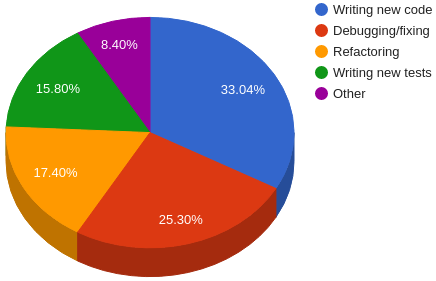
\includegraphics[width=7cm]{images/org-time.png} }}%
        \qquad
        \subfloat[Results in this study]{{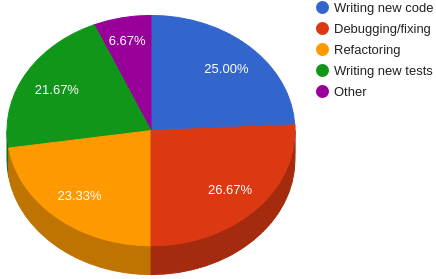
\includegraphics[width=7cm]{images/new-time.png} }}%
        \caption{Developer software development time usage}%
        \label{fig:example}%
    \end{figure}

    \begin{figure}[ht]
      \begin{center}
        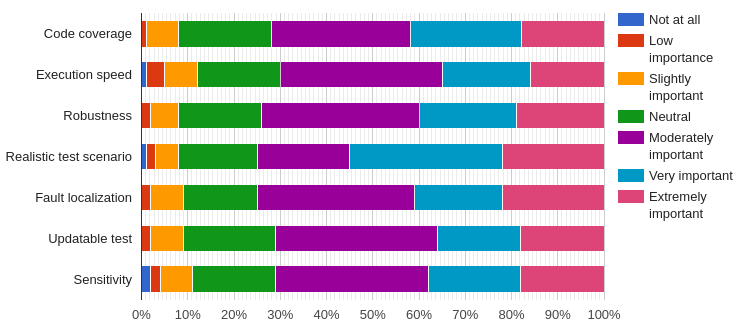
\includegraphics[width=16.7cm]{images/optimize-org.png}
        \caption{Original study~\cite{daka2014survey} unit test optimizing target percentages amongst developers}
        \label{fig:TDD}
      \end{center}
    \end{figure}

    \begin{figure}[ht]
      \begin{center}
        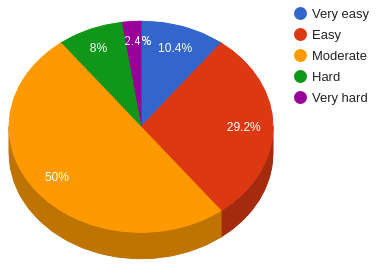
\includegraphics[width=7.7cm]{images/org-understandability.png}
        \caption{Original study~\cite{li2016automatically} unit test understandability}
        \label{fig:TDD}
      \end{center}
    \end{figure}

    \begin{table}[H]
        \resizebox{\textwidth}{!}{%
            \begin{tabular}{p{13.0cm}*{7}{p{2cm}}}
            \topline
            \textbf{Question} & \textbf{Answer options} &  &  &  &   &  & \\ \hline
            \textbf{Q3: How important are the following aspects for you when you write new low-level tests?} & Not at all & Low \newline importance & Slightly important & Neutral & Moderately important & Very \newline important & Extremely important \\
            & \\
            1. Code coverage & 0 & 0 & 0 & {\colorbox{lightgray}A}{\colorbox{lime}B}{\colorbox{orange}C} & 0 & 0 & 0 \\
            2. Capturing all behavior of unit/feature with tests or assertions & 0 & 0 & {\colorbox{lime}B} & {\colorbox{lightgray}A} & 0 & {\colorbox{orange}C} & 0 \\
            3. Execution speed & 0 & {\colorbox{orange}C} & 0 & 0 & {\colorbox{lime}B} & {\colorbox{lightgray}A} & 0 \\
            4. Robustness against code changes (i.e., test does not break easily) & 0 & 0 & 0 & 0 & {\colorbox{lightgray}A}{\colorbox{lime}B}{\colorbox{orange}C} & 0 & 0 \\
            5. How realistic the test scenario is & 0 & 0 & {\colorbox{lightgray}A}{\colorbox{lime}B} & 0 & 0 & {\colorbox{orange}C} & 0 \\
            6. How easily faults can be localised/debugged if the test fails & 0 & 0 & {\colorbox{lime}B} & 0 & {\colorbox{lightgray}A}{\colorbox{orange}C} & 0 & 0 \\
            7. How easily the test can be updated when the underlying code changes & 0 & {\colorbox{orange}C} & {\colorbox{lightgray}A} & 0 & {\colorbox{lime}B} & 0 & 0 \\
            8. Sensitivity against code changes (i.e., test should detect even small code changes) & 0 & {\colorbox{lightgray}A}{\colorbox{lime}B} & 0 & {\colorbox{orange}C} & 0 & 0 & 0 \\
            & \\ \hline
            \textbf{Q3': Compared to JUnit, How important are the following aspects for you when you write new low-level tests?} & A lot less important & Less important & Slightly less important & As important as before & Slightly more important & More important & A lot more important \\
            & \\
            1. Code coverage & 0 & 0 & 0 & {\colorbox{lightgray}A} & 0 & 0 & 0 \\
            2. Capturing all behavior of unit/feature with tests or assertions & 0 & 0 & 0 & 0 & {\colorbox{lightgray}A} & 0 & 0 \\
            3. Execution speed & 0 & 0 & 0 & {\colorbox{lightgray}A} & 0 & 0 & 0 \\
            4. Robustness against code changes (i.e., test does not break easily) & 0 & 0 & 0 & {\colorbox{lightgray}A} & 0 & 0 & 0 \\
            5. How realistic the test scenario is	& 0 & 0 & 0 & {\colorbox{lightgray}A} & 0 & 0 & 0 \\
            6. How easily faults can be localised/debugged if the test fails & 0 & 0 & 0 & 0 & {\colorbox{lightgray}A} & 0 & 0 \\
            7. How easily the test can be updated when the underlying code changes & 0 & 0 & 0 & {\colorbox{lightgray}A} & 0 & 0 & 0 \\
            8. Sensitivity against code changes (i.e., test should detect even small code changes) & 0 & 0 & 0 & {\colorbox{lightgray}A} & 0 & 0 & 0 \\
            & \\ \topline

            \end{tabular}}
            \caption {Optimizing targets in low-level tests and changes in them} \label{tab:changes-pt2}
    \end{table}
    \begin{table}[H]
        \resizebox{\textwidth}{!}{%
            \begin{tabular}{p{13.0cm}*{7}{p{2cm}}}
            \topline
            \textbf{Question} & \textbf{Answer options} &  &  &  &   &  & \\ \hline
            & Very easy & Easy & Moderate & Hard & Very hard & & \\
            & \\
            \textbf{Q4: How difficult is it for you to understand a low-level test?} & 0 & 0 & {\colorbox{lime}B}{\colorbox{orange}C} & {\colorbox{lightgray}A} & 0 \\
            & \\ \hline
            & A lot less difficult & Less difficult & Slightly less difficult & As difficult as before & Slightly more difficult & More difficult & A lot more difficult \\
            & \\
            \textbf{Q4': Compared to JUnit, how difficult is it for you to understand a low-level test?} & 0 & {\colorbox{lightgray}A} & 0 & 0 & 0 & 0 & 0 \\
            & \\ \hline

            \textbf{Q5: In low-level testing, how difficult is it for you to} & Very easy & Easy & Slightly easy & Moderate & Slightly hard & Hard & Very hard \\
            & & & & & & \\
            1. Structure and write information to context of test? & 0 & {\colorbox{lightgray}A} & 0 & 0 & {\colorbox{lime}B}{\colorbox{orange}C} & 0 & 0 \\
            2. Structure and write information to stimulus of test? & 0 & 0 & 0 & {\colorbox{lightgray}A}{\colorbox{lime}B}{\colorbox{orange}C} & 0 & 0 & 0 \\
            3. Structure and write information to assertions of test? & 0 & {\colorbox{lime}B} & {\colorbox{orange}C} & 0 & {\colorbox{lightgray}A} & 0 & 0 \\
            4. Read test case structure for information about context of test? & 0 & 0 & {\colorbox{orange}C} & 0 & {\colorbox{lime}B} & {\colorbox{lightgray}A} & 0 \\
            5. Read test case structure for information about stimulus of test? & 0 & 0 & {\colorbox{orange}C} & {\colorbox{lime}B} & {\colorbox{lightgray}A} & 0 & 0 \\
            6. Read test case structure for information about assertions of test? & 0 & {\colorbox{lime}B} & {\colorbox{orange}C} & 0 & 0 & {\colorbox{lightgray}A} & 0 \\
            & \\ \hline
            \textbf{Q5': Compared to JUnit in low-level testing, how difficult is it for you to} & A lot less difficult & Less difficult & Slightly less difficult & As difficult as before & Slightly more difficult & More difficult & A lot more difficult \\
            & & & & & & \\
            1. Structure and write information to context of test? & {\colorbox{lightgray}A} & 0 & 0 & 0 & 0 & 0 & 0 \\
            2. Structure and write information to stimulus of test? & 0 & {\colorbox{lightgray}A} & 0 & 0 & 0 & 0 & 0 \\
            3. Structure and write information to assertions of test? & 0 & 0 & {\colorbox{lightgray}A} & 0 & 0 & 0 & 0 \\
            4. Read test case structure for information about context of test? & 0 & 0 & {\colorbox{lightgray}A} & 0 & 0 & 0 & 0 \\
            5. Read test case structure for information about stimulus of test? & 0 & {\colorbox{lightgray}A} & 0 & 0 & 0 & 0 & 0 \\
            6. Read test case structure for information about assertions of test? & 0 & 0 & {\colorbox{lightgray}A} & 0 & 0 & 0 & 0 \\
            & \\ \hline

            & Not at all & Hardly informative & Slightly informative & Somewhat informative & Moderately informative & Very informative & Extremely informative \\
            & \\
            \textbf{Q6: How informative you usually find the test case output?} & 0 & {\colorbox{lightgray}A} & 0 & {\colorbox{orange}C} & {\colorbox{lime}B} & 0 & 0 \\
            & \\ \hline
            & A lot less informative & Less informative & Slightly less informative & As informative as before & Slightly more informative & More informative & A lot more informative \\
            & \\
            \textbf{Q6': Compared to JUnit, how informative you usually find the test case output?} & 0 & 0 & 0 & 0 & {\colorbox{lightgray}A} & 0 & 0 \\
            & \\ \topline

            \end{tabular}}
            \caption {Understandability of low-level tests and changes in it} \label{tab:changes-pt3}
    \end{table}
    \begin{table}[H]
        \resizebox{\textwidth}{!}{%
            \begin{tabular}{p{13.0cm}*{7}{p{2cm}}}
            \topline
            \textbf{Question} & \textbf{Answer options} &  &  &  &   &  & \\ \hline
            \textbf{Q7: How much are the following repetition reducing techniques used in your low-level testing?} & Never & Very rarely & Rarely & Occasionally & Frequently & Very \newline frequently & Always \\
            & & & & & & \\
            1. Extract method (custom helper methods) & 0 & 0 & 0 & 0 & {\colorbox{lightgray}A}{\colorbox{lime}B} & {\colorbox{orange}C} & 0 \\
            2. Lifecycle hooks Before/After -class & 0 & 0 & 0 & {\colorbox{orange}C} & {\colorbox{lightgray}A}{\colorbox{lime}B} & 0 & 0 \\
            3. Lifecycle hooks Before/After (each) & 0 & 0 & 0 & 0 & {\colorbox{lightgray}A}{\colorbox{lime}B} & {\colorbox{orange}C} & 0 \\
            4. Automatic test case generation via test case parametrization & 0 & {\colorbox{lightgray}A} & {\colorbox{lime}B} & {\colorbox{orange}C} & 0 & 0 & 0 \\
            5. Common test initializer class inheritance & 0 & {\colorbox{lightgray}A}{\colorbox{orange}C} & {\colorbox{lime}B} & 0 & 0 & 0 & 0 \\
            & \\ \hline

            \textbf{Q7': Compared to JUnit, how much are the following repetition reducing techniques used in your low-level testing?} & A lot less & Less & Slightly less & The same amount & Slightly more & More & A lot more \\
            & & & & & & \\
            1. Extract method (custom helper methods) & 0 & 0 & 0 & {\colorbox{lightgray}A} & 0 & 0 & 0 \\
            2. Lifecycle hooks Before/After -class & 0 & 0 & 0 & {\colorbox{lightgray}A} & 0 & 0 & 0 \\
            3. Lifecycle hooks Before/After (each) & 0 & 0 & 0 & 0 & 0 & {\colorbox{lightgray}A} & 0 \\
            4. Automatic test case generation via test case parametrization & 0 & 0 & 0 & {\colorbox{lightgray}A} & 0 & 0 & 0 \\
            5. Common test initializer class inheritance & 0 & 0 & 0 & {\colorbox{lightgray}A} & 0 & 0 & 0 \\
            & \\ \topline

            \end{tabular}}
            \caption {Used repetition reducing techniques for low-level testing and changes in their use} \label{tab:changes-pt4}
    \end{table}
    \begin{figure}[ht]%
        \centering
        \subfloat[Comment adding ]{{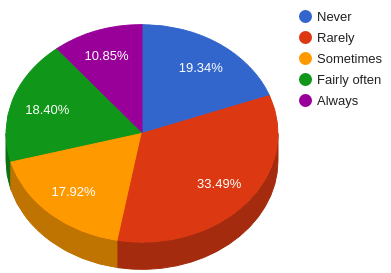
\includegraphics[width=7cm]{images/org-add-document.png} }}%
        \qquad
        \subfloat[Comment updating]{{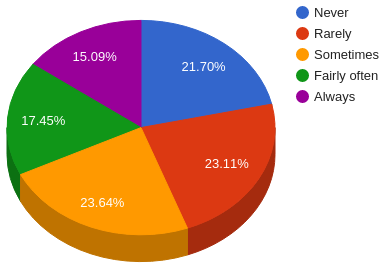
\includegraphics[width=7cm]{images/org-update-document.png} }}%
        \caption{Original study~\cite{li2016automatically} unit testing commenting practices}%
        \label{fig:example}%
    \end{figure}
    \begin{table}[H]
        \resizebox{\textwidth}{!}{%
            \begin{tabular}{p{13.0cm}*{7}{p{2cm}}}
            \topline
            \textbf{Question} & \textbf{Answer options} &  &  &  &   &  & \\ \hline
            & Never & Rarely & Sometimes & Fairly often & Always & & \\
            & \\
            \textbf{Q8: How often do you add/write documentation comments to low-level test cases?} & 0 & {\colorbox{orange}C} & 0 & {\colorbox{lightgray}A}{\colorbox{lime}B} & 0 \\
            & \\ \hline
            & A lot less & Less & Slightly less & The same amount & Slightly more & More & A lot more \\
            & \\
            \textbf{Q8': Compared to JUnit, how often do you add/write documentation comments to low-level test cases?} & 0 & 0 & 0 & 0 & 0 & {\colorbox{lightgray}A} & 0 \\
            & \\ \hline

            & Never & Rarely & Sometimes & Fairly often & Always & & \\
            & \\
            \textbf{Q9: When you make changes to low-level tests, how often do you comment the changes (or update existing comments)?} & 0 & {\colorbox{orange}C} & 0 & {\colorbox{lightgray}A}{\colorbox{lime}B} & 0 \\
            & \\ \hline
            & A lot less & Less & Slightly less & The same amount & Slightly more & More & A lot more \\
            & \\
            \textbf{Q9': Compared to JUnit when you make changes to low-level tests, how often do you comment the changes (or update existing comments)?} & 0 & 0 & 0 & 0 & {\colorbox{lightgray}A} & 0 & 0 \\
            & \\ \topline

            \end{tabular}}
            \caption {Documentation practices in low-level testing and changes in them} \label{tab:changes-pt2}
    \end{table}
    \begin{table}[H]
        \resizebox{\textwidth}{!}{%
            \begin{tabular}{p{13.0cm}*{7}{p{2cm}}}
            \topline
            \textbf{Question} & \textbf{Answer options} &  &  &  &   &  & \\ \hline
            \textbf{Q10: In unit testing, how many} & 0 & 1 & 2-3 & 4-5 & 6-7 &  8-9 & 10 or more \\
            & \\
            1. Test methods do you usually write per class method? & 0 & 0 & {\colorbox{lightgray}A}{\colorbox{lime}B} & {\colorbox{orange}C} & 0 & 0 & 0 \\
            2. Assertions do you usually write per test method? & 0 & 0 & {\colorbox{lightgray}A}{\colorbox{lime}B} & {\colorbox{orange}C} & 0 & 0 & 0 \\
            & \\ \hline
            \textbf{Q10': Compared to JUnit in unit testing} & A lot less & Less & Slightly less & The same amount & Slightly more & More & A lot more \\
            & \\
            1. Do you write more or less test methods per class method? & 0 & 0 & 0 & 0 & 0 & {\colorbox{lightgray}A} & 0 \\
            2. Do you write more or less assertions per test method? & 0 & {\colorbox{lightgray}A} & 0 & 0 & 0 & 0 & 0 \\
            & \\ \hline

            & Mockito & jMock & Powermock & Easymock & Other & & \\
             \\
            \textbf{Q11: In unit testing, what mocking library do you normally use?} & {\colorbox{lightgray}A}{\colorbox{lime}B}{\colorbox{orange}C} & 0 & 0 & 0 & 0 \\
            & \\ \hline
            & \textit Mockito & jMock & Powermock & Easymock & Spock's internal mocking & Other & \\
            & \\
            \textbf{Q11': In unit testing with \textit{Spectrum/Spock}, what mocking library do you normally use?} & {\colorbox{lightgray}A} & 0 & 0 & 0 & 0 & 0 \\
            & \\ \hline

            \textbf{Q12: In unit testing, how difficult you find it to} & Very easy & Easy & Slightly easy & Moderate & Slightly hard & Hard & Very hard \\
            & \\
            1. Mock objects? & 0 & {\colorbox{lime}B}{\colorbox{orange}C} & {\colorbox{lightgray}A} & 0 & 0 & 0 & 0 \\
            2. Stub method calls? & 0 & 0 & {\colorbox{lightgray}A}{\colorbox{orange}C} & 0 & {\colorbox{lime}B} & 0 & 0 \\
            3. Verify mock object actions? & 0 & {\colorbox{lime}B}{\colorbox{orange}C} & 0 & {\colorbox{lightgray}A} & 0 & 0 & 0 \\
            & \\ \hline
            \textbf{Q12': Compared to JUnit in unit testing, how difficult you find it to} & A lot easier & Easier & Slightly easier & As difficult as before & Slightly harder & Harder & A lot harder \\
            & \\
            1. Mock objects? & 0 & 0 & 0 & 0 & {\colorbox{lightgray}A} & 0 & 0 \\
            2. Stub method calls? & 0 & 0 & 0 & 0 & {\colorbox{lightgray}A} & 0 & 0 \\
            3. Verify mock object actions? & 0 & 0 & 0 & 0 & {\colorbox{lightgray}A} & 0 & 0 \\
            & \\ \hline

            & Before implementation & During implementation & After implementation & \\
            & \\
            \textbf{Q13: When do you add automated unit tests for developed code with \textit{JUnit}?} & 0 & {\colorbox{lime}B}{\colorbox{orange}C} & {\colorbox{lightgray}A} \\
            & \\ \hline
            & Before implementation & During implementation & After implementation & \\
            & \\
            \textbf{Q13': When do you add automated unit tests for developed code with \textit{Spectrum/Spock}?} & 0 & 0 & {\colorbox{lightgray}A} \\
            & \\ \topline

            \end{tabular}}
            \caption {Unit testing practices and changes in them} \label{tab:junit-pt1}
    \end{table}
    \clearpage

\subsection{Developer perception towards automated low-level testing}
    \begin{figure}[ht]
      \begin{center}
        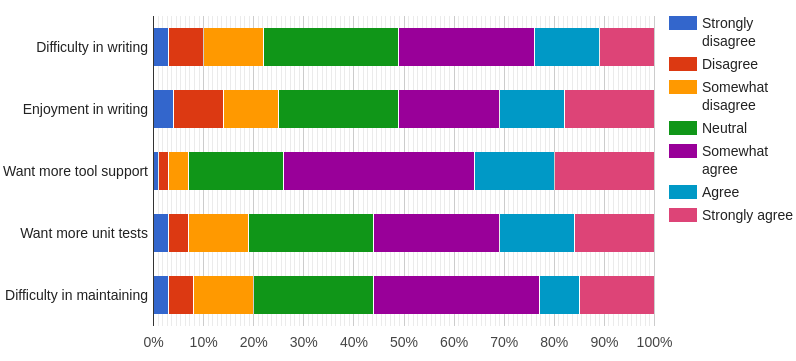
\includegraphics[width=14.7cm]{images/perception-org.png}
        \caption{Original study~\cite{daka2014survey} developer perception of unit testing}
        \label{fig:TDD}
      \end{center}
    \end{figure}

    \begin{figure}[ht]%
        \centering
        \subfloat[Unit tests help in producing higher quality code~\cite{williams2009effectiveness}]{{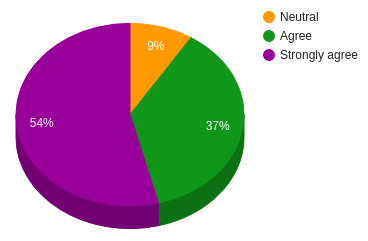
\includegraphics[width=7cm]{images/org-quality.png} }}%
        \qquad
        \subfloat[Maintaining unit tests is important for the quality of the system~\cite{li2016automatically}]{{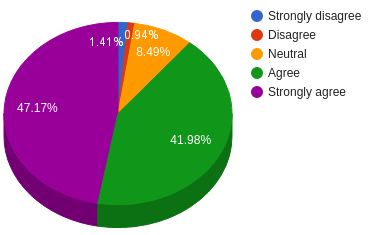
\includegraphics[width=7cm]{images/org-maintaining.png} }}%
        \caption{Developer perception of unit testing in original studies}%
        \label{fig:example}%
    \end{figure}

    \begin{table}[H]
        \resizebox{\textwidth}{!}{%
            \begin{tabular}{p{13.0cm}*{7}{p{2cm}}}
            \topline
            \textbf{Question} & \textbf{Answer options} &  &  &  &   &  & \\ \hline

            \textbf{Q14: Please indicate your level of agreement with the following statements} & Strongly disagree & Disagree & Somewhat disagree & Neither agree nor disagree & Somewhat agree & Agree & Strongly agree \\
            & \\
            1. Writing low-level tests is difficult & 0 & 0 & {\colorbox{orange}C} & 0 & {\colorbox{lightgray}A}{\colorbox{lime}B} & 0 & 0 \\
            2. I enjoy writing low-level tests & 0 & {\colorbox{lime}B} & 0 & {\colorbox{lightgray}A} & 0 & {\colorbox{orange}C} & 0 \\
            3. I would like to have more tool support when writing low-level tests & 0 & 0 & {\colorbox{lime}B} & {\colorbox{lightgray}A} & {\colorbox{orange}C} & 0 & 0 \\
            4. I would like to have more low-level tests & 0 & 0 & 0 & {\colorbox{lightgray}A}{\colorbox{lime}B}{\colorbox{orange}C} & 0 & 0 & 0 \\
            5. Maintaining low-level tests is difficult & 0 & 0 & {\colorbox{orange}C} & 0 & {\colorbox{lime}B} & {\colorbox{lightgray}A} & 0 \\
            6. I think my low-level tests will help other developers to understand the implemented unit/feature better & 0 & 0 & {\colorbox{lime}B} & 0 & {\colorbox{lightgray}A} & {\colorbox{orange}C} & 0 \\
            7. Low-level automated testing helps me find defects in the code before other quality assurance phases & 0 & 0 & 0 & 0 & {\colorbox{lime}B} & {\colorbox{orange}C} & {\colorbox{lightgray}A} \\
            8. JUnit promotes me to write high quality test code & 0 & 0 & {\colorbox{lightgray}A}{\colorbox{orange}C} & {\colorbox{lime}B} & 0 & 0 & 0 \\
            & \\ \hline

            \textbf{Q15a: Please indicate your level of agreement with the following statements} & Strongly disagree & Disagree & Neutral & Agree & Strongly agree & \\
            & \\
            1. Overall, low-level tests help me produce higher quality code & 0 & 0 & 0 & {\colorbox{lime}B} & {\colorbox{lightgray}A}{\colorbox{orange}C} \\
            2. Maintaining good low-level test cases and their documentations is important to the quality of a system & 0 & 0 & 0 & {\colorbox{lightgray}A}{\colorbox{lime}B} & {\colorbox{orange}C} \\
            & \\ \topline

            \end{tabular}}
            \caption {Developer perception of low-level testing with JUnit} \label{tab:junit-pt2}
    \end{table}

    \begin{table}[H]
        \resizebox{\textwidth}{!}{%
            \begin{tabular}{p{13.0cm}*{7}{p{2cm}}}
            \topline
            \textbf{Question} & \textbf{Answer options} &  &  &  &   &  & \\ \hline
            \textbf{Q14'\&Q15a': Please indicate your level of agreement with the following statements} & Strongly disagree & Disagree & Somewhat disagree & Neither agree nor disagree & Somewhat agree & Agree & Strongly agree \\
            & \\
            1. Writing low-level tests with \textit{Spectrum/Spock} is more difficult than with JUnit & 0 & 0 & 0 & 0 & {\colorbox{lightgray}A} & 0 & 0 \\
            2. I enjoy writing low-level tests with \textit{Spectrum/Spock} more than I do with JUnit & 0 & 0 & 0 & 0 & {\colorbox{lightgray}A} & 0 & 0 \\
            3. I would like to have more tool support for \textit{Spectrum/Spock} when writing low-level tests & 0 & 0 & 0 & 0 & 0 & 0 & {\colorbox{lightgray}A} \\
            4. I would like to have more low-level tests for \textit{Spectrum/Spock} & 0 & 0 & 0 & 0 & {\colorbox{lightgray}A} & 0 & 0 \\
            5. Maintaining low-level tests with \textit{Spectrum/Spock} is more difficult than with JUnit & 0 & 0 & 0 & 0 & {\colorbox{lightgray}A} & 0 & 0 \\
            6. I think my low-level tests with \textit{Spectrum/Spock} will help other developers to understand the implemented unit/feature better than earlier tests with JUnit & 0 & 0 & 0 & 0 & 0 & {\colorbox{lightgray}A} & 0 \\
            7. Low-level automated testing with \textit{Spectrum/Spock} helps me find defects in the code before other quality assurance phases better than earlier tests with JUnit & 0 & 0 &  {\colorbox{lightgray}A} & 0 & 0 & 0 & 0 \\
            8. \textit{Spectrum/Spock} promotes me to write higher quality test code than with JUnit & 0 & 0 & 0 & 0 & 0 &  {\colorbox{lightgray}A} & 0 \\ \hline
            & \\
            9. Overall, low-level tests with \textit{Spectrum/Spock} help me produce higher quality code than with JUnit & 0 & 0 &  {\colorbox{lightgray}A} & 0 & 0 & 0 & 0 \\
            10. Maintaining good low-level test cases and their documentation with \textit{Spectrum/Spock} is more important for system quality than maintaining JUnit test cases & 0 & 0 & 0 & 0 & {\colorbox{lightgray}A} & 0 & 0 \\
            & \\ \topline

            \end{tabular}}
            \caption {Developer perception changes in low-level testing with \textit{Spectrum/Spock}} \label{tab:junit-pt2}
    \end{table}
    \vspace{20px}


    \begin{table}[H]
        \resizebox{\textwidth}{!}{%
            \begin{tabular}{p{15.0cm}*{3}{p{2.0cm}}}
            \topline
            \textbf{Question} & \textbf{Answer options} &  &  \\ \hline

            \textbf{Q15b: I would say that I write more} & Yes & Uncertain & No \\
            & \\
            1. Understandable low-level tests with \textit{Spectrum/Spock} than with JUnit? & {\colorbox{lightgray}A} & 0 & 0 \\
            2. Maintainable low-level tests with \textit{Spectrum/Spock} than with JUnit? & {\colorbox{lightgray}A} & 0 & 0  \\
            & \\ \topline

            \end{tabular}}
            \caption {Developer perception towards \textit{Spectrum/Spock}} \label{tab:spock-spectrum-pt3}

    \end{table}

    \begin{table}[H]
        \resizebox{\textwidth}{!}{%
            \begin{tabular}{p{17.0cm}*{11}{p{1cm}}}
            \topline
            \textbf{Question} & \multicolumn{3}{l}{\textbf{Answer options}} & \\
            & \\ \hline
            & \multicolumn{4}{l}{\textit{Not at all likely}} & & & & \multicolumn{4}{r}{\textit{Extremely likely}} \\
            \textbf{Q16: How likely are you to} & 0 & 1 & 2 & 3 & 4 & 5 & 6 & 7 & 8 & 9 & 10 \\
            & \\
            1. Recommend low-level automated testing for colleague as a software development practice? & 0 & 0 & 0 & 0 & 0 & 0 & 0 & 0 & {\colorbox{lime}B} & 0 & {\colorbox{lightgray}A}{\colorbox{orange}C} \\
            2. Recommend testing framework JUnit for future Spring projects where you take part in existing project? & 0 & 0 & 0 & 0 & 0 & 0 & 0 & {\colorbox{orange}C} & 0 & {\colorbox{lime}B} & {\colorbox{lightgray}A} \\
            3. Take testing framework JUnit in use for future Spring projects where you have technical lead role in a new starting project? & 0 & 0 & 0 & 0 & 0 & 0 & 0 & 0 & {\colorbox{orange}C} & {\colorbox{lime}B} & {\colorbox{lightgray}A} \\
            & \\ \hline
            & \multicolumn{4}{l}{\textit{Not at all likely}} & & & & \multicolumn{4}{r}{\textit{Extremely likely}} \\
            \textbf{Q16': How likely are you to} & 0 & 1 & 2 & 3 & 4 & 5 & 6 & 7 & 8 & 9 & 10 \\
            & \\
            1. Recommend low-level automated testing for colleague as a software development practice? & 0 & 0 & 0 & 0 & 0 & 0 & 0 & 0 & 0 & 0 & {\colorbox{lightgray}A} \\
            2. Recommend testing framework \textit{Spectrum/Spock} for future Spring projects where you take part in existing project? & 0 & 0 & 0 & 0 & 0 & 0 & {\colorbox{lightgray}A} & 0 & 0 & 0 & 0 \\
            3. Take testing framework \textit{Spectrum/Spock} in use for future Spring projects where you have technical lead role in a new starting project? & 0 & 0 & 0 & 0 & 0 & 0 & {\colorbox{lightgray}A} & 0 & 0 & 0 & 0 \\
            & \\ \topline

            \end{tabular}}
            \caption {NPS questions related to JUnit and \textit{Spectrum/Spock}} \label{tab:junit-pt3}

    \end{table}

    \clearpage
\restoregeometry

\section{Test code analysis}
Test code analysis was done to answer \textbf{RQ3} with metrics defined in chapter \ref{chapter:methods} section \ref{subsub:test}.
Test code analysis was done with master branches of projects A and B, \textbf{before} and \textbf{after} the introduction of new BDD testing framework, to related
low-level tests and their affected components. First the unit testing level changes are inspected with projects A and B.
After this, the low-level testing metrics and changes in them are demonstrated with both projects.

\subsection{Automated unit testing level}
At automated unit testing level, two metrics were used to study the changes in unit testing: average \textbf{count of test methods}
per tested class methods and \textbf{code coverage}. Table \ref{tab:unit-metrics} displays these values before the introduction
of new BDD testing framework and after. In \textbf{COTM} before values are calculated for JUnit unit tests only and after
values only for new unit tests done with the selected BDD testing framework. In \textbf{CC}, before values are for the
whole project at unit level with JUnit. After values are unit testing coverage for JUnit and new BDD testing framework
combined.

{\renewcommand{\arraystretch}{1.3}
\begin{table}[H]
    \resizebox{\textwidth}{!}{%
        \begin{tabular}{p{6.0cm}*{4}{p{3cm}}}

        \headcol \textbf{Metric} & \textbf{Project A} \newline JUnit & \textbf{Project A} \newline Spectrum & \textbf{Project B} \newline JUnit & \textbf{Project B} \newline Spock  \\ \hline

        \rowcol \textit{\textbf{COTM}} & \textbf{1.44} & & \textbf{3.49} & \\
        \rowcol \textit{Sum of tested class methods} & 61 &  & 93 & \\
        \rowcol \textit{Sum of unit test methods} & 88 & & 325 & \\ \hline

        \textit{\textbf{Instruction CC}} & \textbf{25\%} & & \textbf{20\%} & \\
        \textit{Total number of instructions} & 31,425 & & 49,895 & \\
        \textit{\textbf{Branch CC}} & \textbf{24\%} & & \textbf{20\%} & \\
        \textit{Total number of branches} & 724 & & 2,195 & \\ \bottomlinec
        \end{tabular}}
        \caption {Unit level testing metrics in projects and their change} \label{tab:unit-metrics}

\end{table}
}

\textbf{RQ3: }\textit{How does behavior driven testing frameworks change written low-level test cases and test code coverage compared to JUnit framework?}
is first studied with data from unit testing metrics displayed in table \ref{tab:unit-metrics}.

\clearpage
\subsection{Automated unit \& integration testing levels}
At automated low-level testing level there were 5 inspected metrics: \textbf{code coverage}, average \textbf{count of assertions} per test method,
average \textbf{count of comments} per test method, average \textbf{test method name word count} and ratio of \textbf{data driven test methods} to
all low-level test methods. \textbf{CC} is measured as combined JUnit and new BDD framework coverage. All other metrics
are measured first from existing low-level JUnit tests and after from new BDD testing framework specifications.
Table \ref{tab:low-metrics} dislays the values of these metrics in projects A and B before and after introduction of BDD testing framework.


{\renewcommand{\arraystretch}{1.3}
\begin{table}[H]
    \resizebox{\textwidth}{!} & & \textbf{47\%} & \\
        \rowcol \textit{Total number of instructions} & 31,425 & & 49,895 & \\
        \rowcol \textit{\textbf{Branch CC}} & \textbf{54\%} & & \textbf{39\%} & \\
        \rowcol \textit{Total number of branches} & 724 & & 2,195 & \\ \hline

        \textit{\textbf{COA}} & \textbf{2.64} & & \textbf{2.82} & \\
        \textit{Sum of assertions} & 493 & & 1,311 & \\
        \textit{Sum of test methods} & 187 & & 465 & \\ \hline

        \rowcol \textit{\textbf{COC}} & \textbf{1.17} & & \textbf{0.04} & \\
        \rowcol \textit{Sum of comments} & 218 & & 20 & \\
        \rowcol \textit{Sum of test methods} & 187 & & 465 & \\ \hline

        \textit{\textbf{TMNWC}} & \textbf{4.66} & & \textbf{5.61} & \\
        \textit{Total words in test method names} & 872 & & 2,607 & \\
        \textit{Sum of test methods} & 187 & & 465 & \\ \hline

        \rowcol \textit{\textbf{DDTM}} & \textbf{0} & & \textbf{0.02} & \\
        \rowcol \textit{Sum of data driven test methods} & 0 & & 8 & \\
        \rowcol \textit{Sum of test methods} & 187 & & 465 & \\ \bottomlinec

        \end{tabular}}
        \caption {Low-level testing metrics in projects and their change} \label{tab:low-metrics}

\end{table}
}

\textbf{RQ3} can be further analyzed for low-level testing with metrics displayed in table \ref{tab:low-metrics}.

\section{Comparison of BDD testing frameworks}

